
%mainfile: Networks.tex

\pagestyle{fancy} 
\lhead{Atelier Nueromodélisation, 2017}
\rhead{Problem set \#4}
\rfoot{\thepage}
\cfoot{}
\lfoot{~\theauthor}
\renewcommand{\headrulewidth}{0.4pt}
\renewcommand{\footrulewidth}{0.4pt}


\title{Problem Set \#4: Networks \vspace{-0.5em}}
%\preauthor{} \postauthor{} 
\author{Hsieh Yu-Guan}
\date{\today}
\maketitle

\thispagestyle{fancy}

\section*{Introduction}

Besides studying the strucutre and function of a single neuron, it's also
important to understand what may happen when neurons communicate between them.
In this report we'll thus look at some simple models of neural networks.
What will be their dynamics and expressive power? 
(P.S. we'll ignore all physical units for the whole report.)

\section{Some simple networks}

\subsection{Neuron with autapse}

Let's start by working on the simplest model that one can ever imagine:
there's only one neuron in the network, and its output feeds back onto 
itself via a synapse (such a synapse is called an ``autapse''). 
We note $x$ the neuron's firing rate, and it obeys the equation

\[\dot{x}(t) = -x(t) + f(wx(t)+I)\]

\noindent
where $w = 0.04$ is the strength of the synaptic connection and $I = -2$ 
is the external (and inhibitory) background input which is constant.
Finally, $f$ is the input-output (or activation) function of the neuron having
a sigmoidal form and is given by

\[f(s) = 50(1 + tanh(s))\]

\noindent
where $s$ is the total input of the neuron.

To see that $f$ is indeed a sigmoidal function, we plot it for the range 
$s \in [-10, 10]$ as shown in \autoref{fig: activate}. Next, we plot the
derivative of the firing rate $\dot{x}$ as a function of $x$ 
(\autoref{fig: x_derivative}). The form should be easily predictable.
The function $f$ is first stretched out and then shifted to the right,
before we finally add the linear function $x \mapsto -x$ to it.

We observe three zero-crossings in this graph. Let's call them respectively
$x_1$, $x_2$ and $x_3$ with $x_1 < x_2 < x_3$. In fact we get $x_1 \sim 2$,
$x_2 = 50$ and $x_3 \sim 98$. They are the fixed points of the dynamics.
However, $x_1$ and $x_3$ are stable while $x_2$ is unstable.
We can see that if $x$ lies between $x_1$ and $x_2$, $\dot{x}$ is negative
so $x$ will be ``attract'' to $x_1$, and if $x$ is smaller than $x_1$,
$\dot{x}$ is positive and $x$ will converge to $x_1$. The same analysis
works for $x_3$.

\newpage

\vspace{-1em}
\begin{figure}[H]
  \centering
  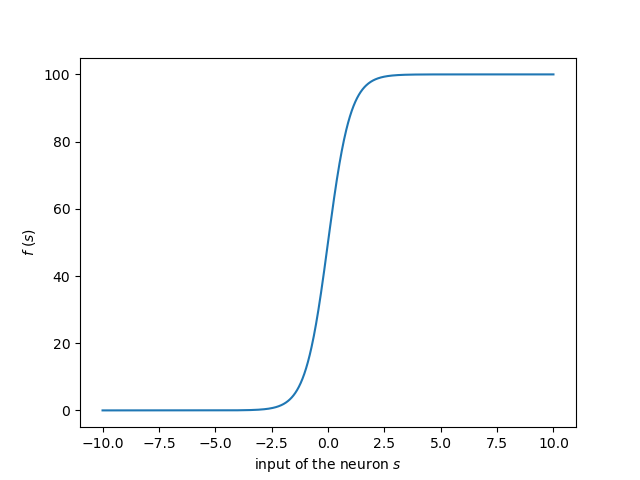
\includegraphics[width=0.7\linewidth]{autapse1}
  \caption{The activtion function $f$ of the neuron}
  \label{fig: activate}
\end{figure}

\vspace{-1em}
\begin{figure}[H]
  \centering
  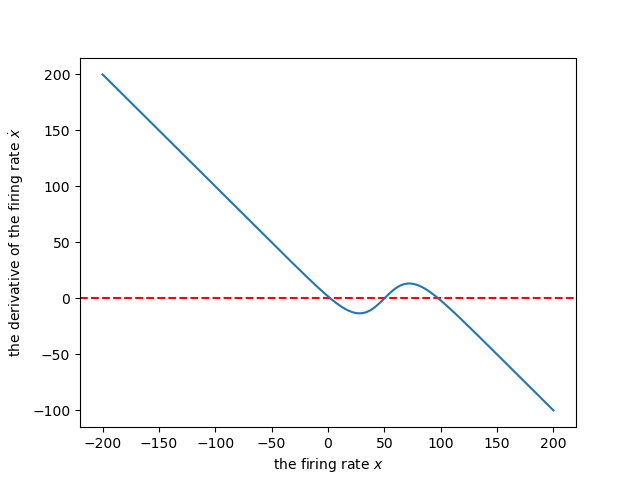
\includegraphics[width=0.7\linewidth]{autapse2}
  \caption{$\dot(x)$ as a function of $x$}
  \label{fig: x_derivative}
\end{figure}

Now we'll simulate the dynamics of the system by taking a time step 
$\Delta t = 0.1$ and a total time period $T = 100$. First consider
$x(0) = 49$.

\vspace{-1em}
\begin{figure}[H]
  \centering
  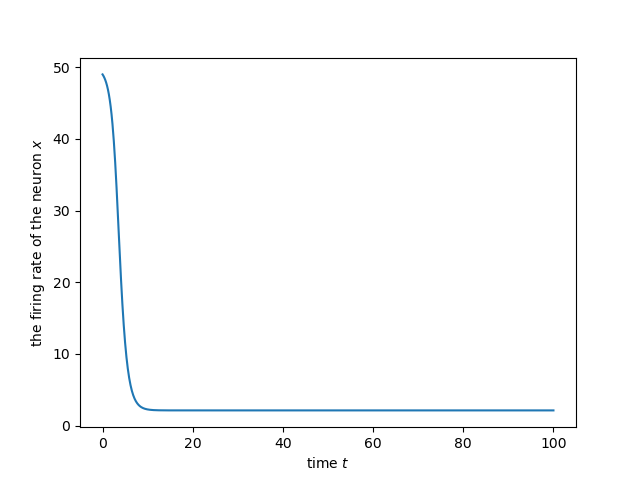
\includegraphics[width=0.7\linewidth]{autapse3}
  \caption{The evolution of $x$ for $x(0) = 49$}
\end{figure}

\noindent
As predicted before $x$ is attracted to the dynamics attractor $x_1$.
We redo the simulation for $x(0) = 50$.

\vspace{-1em}
\begin{figure}[H]
  \centering
  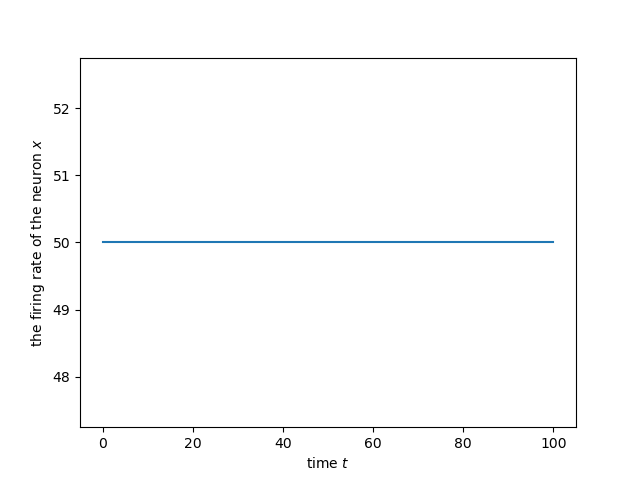
\includegraphics[width=0.7\linewidth]{autapse4}
  \caption{The evolution of $x$ for $x(0) = 50$}
\end{figure}

\noindent
This time since 50 is itself a fixed point of the dynamics, the system 
is at equilibrium and the solution doesn't change with time (though 50
is a repeller). Finally let $x(0) = 51$.

\vspace{-1em}
\begin{figure}[H]
  \centering
  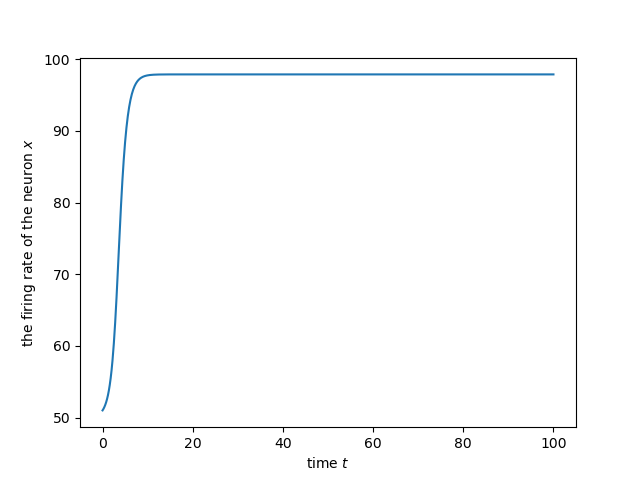
\includegraphics[width=0.7\linewidth]{autapse5}
  \caption{The evolution of $x$ for $x(0) = 51$}
\end{figure}

\noindent
It's the symmetry of the case $x(0) = 49$. Between the repeller $x_2$ and
the attractor $x_3$, $x$ evolves towards $x_3$.

We then add noise to the system, so the differential equation becomes

\[\dot{x}(t) = -x(t) + f(wx(t)+I) + \sigma\eta(t)\]

\noindent
where $\sigma(t)$ is Gaussian white noise with varaiance 1. First we suppose 
$\sigma = 5$ and we simulate for $x(0) = 49$.

\vspace{-1em}
\begin{figure}[H]
  \centering
  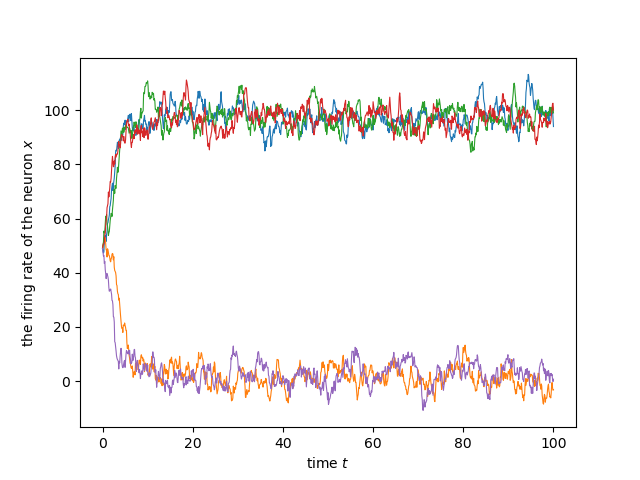
\includegraphics[width=0.7\linewidth]{autapse6}
  \caption{The evolution of $x$ with noise $\sigma = 5$ for $x(0) = 49$}
\end{figure}

We see that there are two different scinarios. With noise we can no longer
ensure that the system will converge towards $x_1$. Since the evolutions of
the system are very different for $x < 50$ and $x > 50$, and 49 is close
to 50, slight noise in the model may lead to totaly distinct results. This can
be again shown for $x(0) = 50$ and $x(0) = 51$.

\vspace{-1em}
\begin{figure}[H]
  \centering
  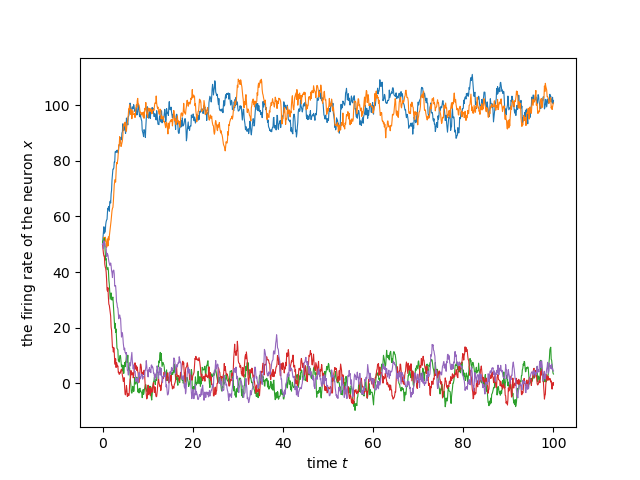
\includegraphics[width=0.7\linewidth]{autapse7}
  \caption{The evolution of $x$ with noise $\sigma = 5$ for $x(0) = 50$}
\end{figure}

\vspace{-1em}
\begin{figure}[H]
  \centering
  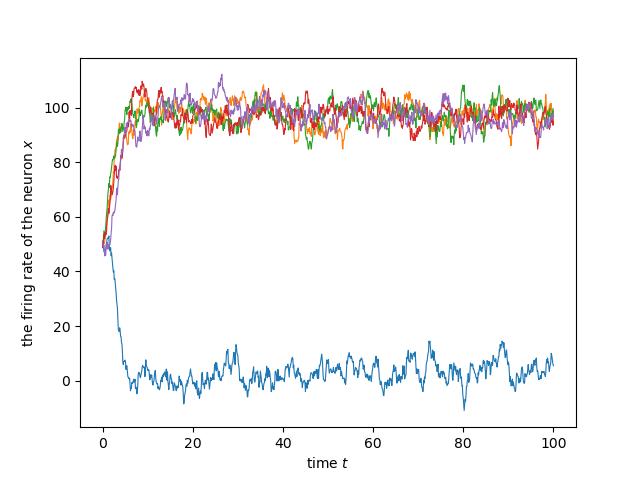
\includegraphics[width=0.7\linewidth]{autapse8}
  \caption{The evolution of $x$ with noise $\sigma = 5$ for $x(0) = 51$}
\end{figure}

Also notice that for $x(0) = 50$, $x$ will not stay anymore at the value 50 
because as mentioned before, $x_2 = 50$ is a repeller. In a model with noise,
the probability that $x$ is always 50 becomes null. 

In all the above examples, though noise can have great influence on the 
evolution of the system, once $x$ gets far enough from $x_2$, the evolution
is still mainly dominated by the drift term $-x(t) + f(wx(t)+I)$.
Nonetheless, this is not the case for a greater noise level, for example,
when $\sigma = 80$, as shown in the top of the next page.

\vspace{-1em}
\begin{figure}[H]
  \centering
  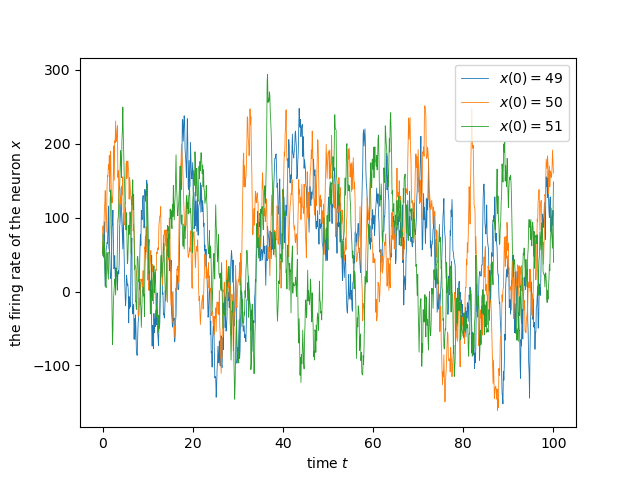
\includegraphics[width=0.7\linewidth]{autapse9}
  \caption
    {The evolution of $x$ with noise $\sigma = 80$ for $x(0) = 49, 50, 51$}
\end{figure}

As the resulting curves follow almost the same pattern for different 
initial values of $x$, I plot all of them on the same graph. It's not worth
it to plot several simulations for a same $x(0)$ because we would not be able
to see great differences. In short, the evolution of $x$ is donimated by
the noise term and becomes just noisy.

\subsection{Circuit with mutual inhibition}

The second model we'll discuss here is made up of two neurons that are coupled
by mutual inhibition. We note the firing rate of the two neurons respectively
$x_1$ and $x_2$, then the whole system is governed by the differential
equations

\begin{gather*}
  \dot{x}_1 = -x_1(t) + f(wx_2(t) + I)\\
  \dot{x}_2 = -x_2(t) + f(wx_1(t) + I)
\end{gather*}

\noindent
where $f$ is defined as before and the inhibitory synaptic weights are given
by $w = 0.1$. The external inputs are now excitatory, $I = 5$.

We may also want to use the vector notation that would turn out to be quite
useful when the population of neurons gets larger, then the system of
differential equations can be put in the form:

\[\dot{\mathbf{x}} = -\mathbf{x}(t) + f(\mathbf{Wx}(t) + \mathbf{I})\]

\noindent
where $\mathbf{x}$ is the vector of firing rates, $\mathbf{W}$ is the synaptic 
weight matrix and $\mathbf{I}$ is the vector of input currents. In this
particular case, we have

\[
  \mathbf{x}(t) = \left(
    \begin{array}{c}
      x_1(t)\\
      x_2(t)
    \end{array}\right) \qquad
  %
  \mathbf{W} = \left(
    \begin{array}{cc}
      0 & w\\
      w & 0
    \end{array}\right) \qquad
  %
  \mathbf{I} = \left(
    \begin{array}{c}
      I\\
      I
    \end{array}\right).
\]

To study the dynamics of this system, we first plot its nullclines, that is,
the line for which $\dot{x}_1(t)=0$ and the line for which $\dot{x}_2(t)=0$.

\begin{figure}[H]
  \centering
  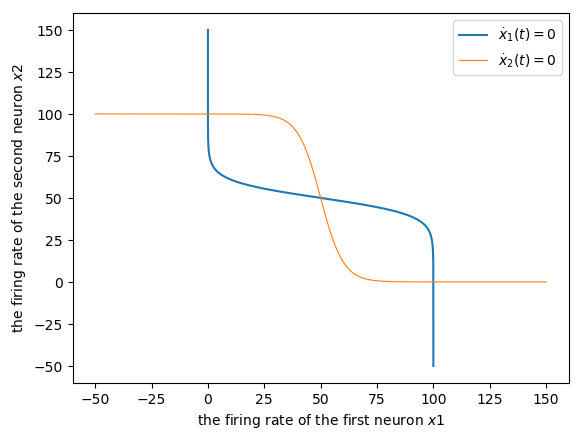
\includegraphics[width=0.7\linewidth]{mutual1}
  \caption
    {The nullclines of the system of two mutual inhibitory neurons}
\end{figure}

We observe three crossing points of the the two lines. From left to right,
we name them respectively $z_1$, $z_2$ and $z_3$ (so $z_2 = (50,50)$).
These are the points such that $\dot{x}_1 = \dot{x}_2 = 0$. In other words,
they're the fixed points of the dynamics. The plane is then divided into six
zones and in each zone the system evolves in a specific direction. To put it
simply, on the left of the blue line we have $\dot{x}_1 > 0$ while on the
right $\dot{x}_1 < 0$. Similarly, below the orange line we get
$\dot{x}_2 > 0$ whereas above it $\dot{x}_2 < 0$.

To better undestand what this implies, we simulate the system and plot the 
evolution of the firing rates for different initial conditions in the figure 
below.

\begin{figure}[H]
  \centering
  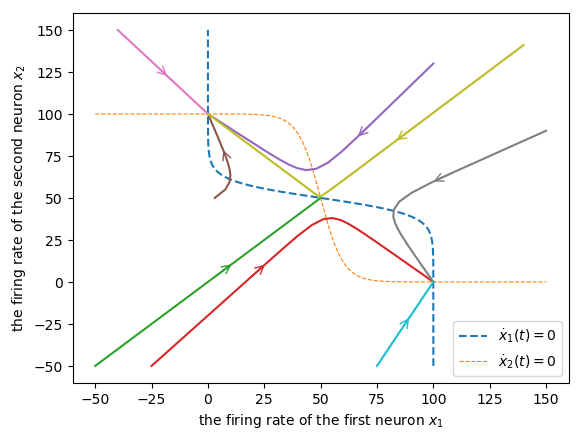
\includegraphics[width=0.7\linewidth]{mutual2}
  \caption
    {The evolution of the firing rates for different initial conditions}
\end{figure}

The initial conditions that are considered here are $(-50, -50)$, $(-40, 150)$,
$(-25, 50)$, $(3, 50)$, $(75, -50)$, $(100, 130)$, $(140, 141)$ and 
$(150, 90)$. First we notice that all of the simulations end up in some fixed
point and the directions of the evolutions follow roughly what is described
above. Further, it seems that (but without rigorous mathematical proof here)
given the initial condition $(x(0),y(0))$, if $x(0) < y(0)$ the system evolves
to $z_1$; if $x(0) = y(0)$ the system converges to $z_2$; finally if 
$x(0) > y(0)$ the system moves to $z_3$.

The yellow arrow serves as quite a good example: the initial condition is 
$(150, 151)$, and the system gets once very clear to $z_2$ but then it again
leaves away from this point and converges to $z_1$ at the end. As a result,
being fixed point, $z_1$ and $z_3$ are stable while $z_2$ is unstable. 
Finally, a plot of the vector field of derivatives can better 
explain all of this.

\begin{figure}[H]
  \centering
  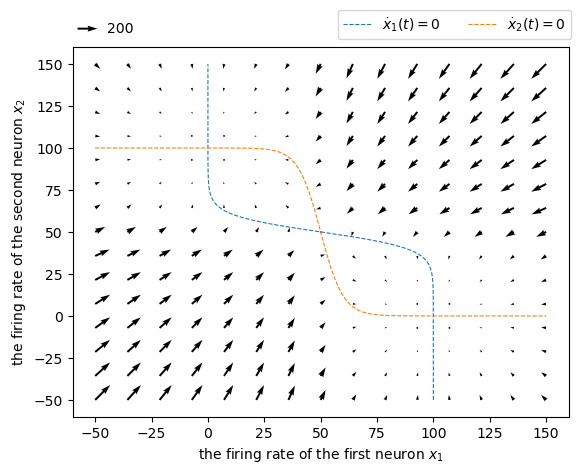
\includegraphics[width=0.7\linewidth]{mutual3}
  \caption
    {Derivatives at some points of the system}
\end{figure}

\subsection{Conclusion}
In this section, we have investigated two relatively simple networks and spent
time studying their dynamics. Several simulations have also been carried out.
We saw that there are diffrent kinds of fixed points of dynamics and if the
external currents are constant, the system will evolve towards some final 
state (which is often an attractor). Finally, the presence of noise may more
or less affect the evolution of the system.

